\documentclass[11pt]{article}
\usepackage[margin=1in]{geometry} 
\usepackage{amsmath,amsthm,amssymb,amsfonts}
\usepackage{graphicx} % figures
\usepackage{subcaption} % multi subplots 
\usepackage{multirow} % table

\usepackage{biblatex}
\addbibresource{MyRef.bib}

\graphicspath{{figures/}}

\begin{document}
\title{Machine Learning Practical \\Assignment 2}

\author{Siyuan Zhao}
\maketitle
\section{Combining L1 and L2 regularisation}

\subsection{Experimental hypothesis}
In this section, An investigation was conducted to evaluate the method of combining L1 and L2 regularisation on overcoming the problem of overfitting. The method is also compared to L1 and L2 regularisation individually. The goal is to find whether combining L1 and L2 regularisation can offer any advantage over using either individually?

\subsection{Methodology}
As L1 and L2, an complexity term $E_w$ will be added to the error function.
\begin{equation}
	E^n = E_{train}^n + E_w
\end{equation}
To combine L1 and L2 regularisation, the term of $E_w$ should included both the L1 term of $|w_i|$ and L2 term of $\frac{1}{2}w_i^2$. A linear relationship is applied here where $\alpha$ and $\beta$ is the coefficient control the L1 and L2 term.
\begin{equation}
	E_w = \alpha \sum_i|w_i| + \beta \frac{1}{2}\sum_iw_i^2
\end{equation}
This has a gradient with respect to the parameter vector
\begin{equation}
	\frac{\partial E_w}{\partial w_i} = \alpha sgn(w_i) + \beta w_i
\end{equation}
where $\textrm{sgn}(u) = +1$ if $u > 0$, $\textrm{sgn}(u) = -1$ if $u < 0$ (and is not well defined for $u=0$ though a common convention is to have $\textrm{sgn}(0) = 0$).
the total error with respect to the parametrs
\subsection{Implementation and Results}
In the python notebook file {\bf CW2}, a class called {\bf L1\_L2\_Penalty} is developed according to the definition of the method of new regularisation. The remaining part of the python notebook is about three plots. The first plot is the training and validation error against various values of coefficients for L1 term and L2 term. The second plot is the training and validation error against epoch number for all different regularisation schemes on the same axis. The third plot is about comparison between individual L1 and L2 regularisation, L1 and L2 combination regularisation and the model without regularisation. 
In this experiment 
\begin{table}
\begin{center}
\begin{tabular}{ c  c c c c  c c} 
\hline
coeff\_L1 & coeff\_L2 &error(train) & error(valid) & acc(train) & acc(valid) & params\_penalty\\
\hline
\hline
1e-07& 1e-06	&1.53e-04 & 1.22e-01 & 1.00e+00 & 9.79e-01 &7.05e-04\\ 
1e-06 & 1e-05  	&3.87e-04 & 1.03e-01 & 1.00e+00 & 9.80e-01 &5.81e-03\\ 
1e-05 &1e-04	 &4.39e-03 & 7.21e-02 & 1.00e+00 & 9.80e-01 &3.38e-02\\ 
1e-04 & 1e-03 & 6.13e-02  &  8.31e-02  &  9.83e-01 & 9.76e-01  &  1.39e-01\\
1e-03 & 1e-02 &3.37e-01&  3.06e-01   & 9.09e-01 & 9.21e-01 &4.13e-01\\
\end{tabular}
\caption{Performance of different coefficients for combining method for L1 and L2}
\label{tb:L1_L2_combine}
\end{center}	
\end{table}

\begin{figure}[h]
\centering 
  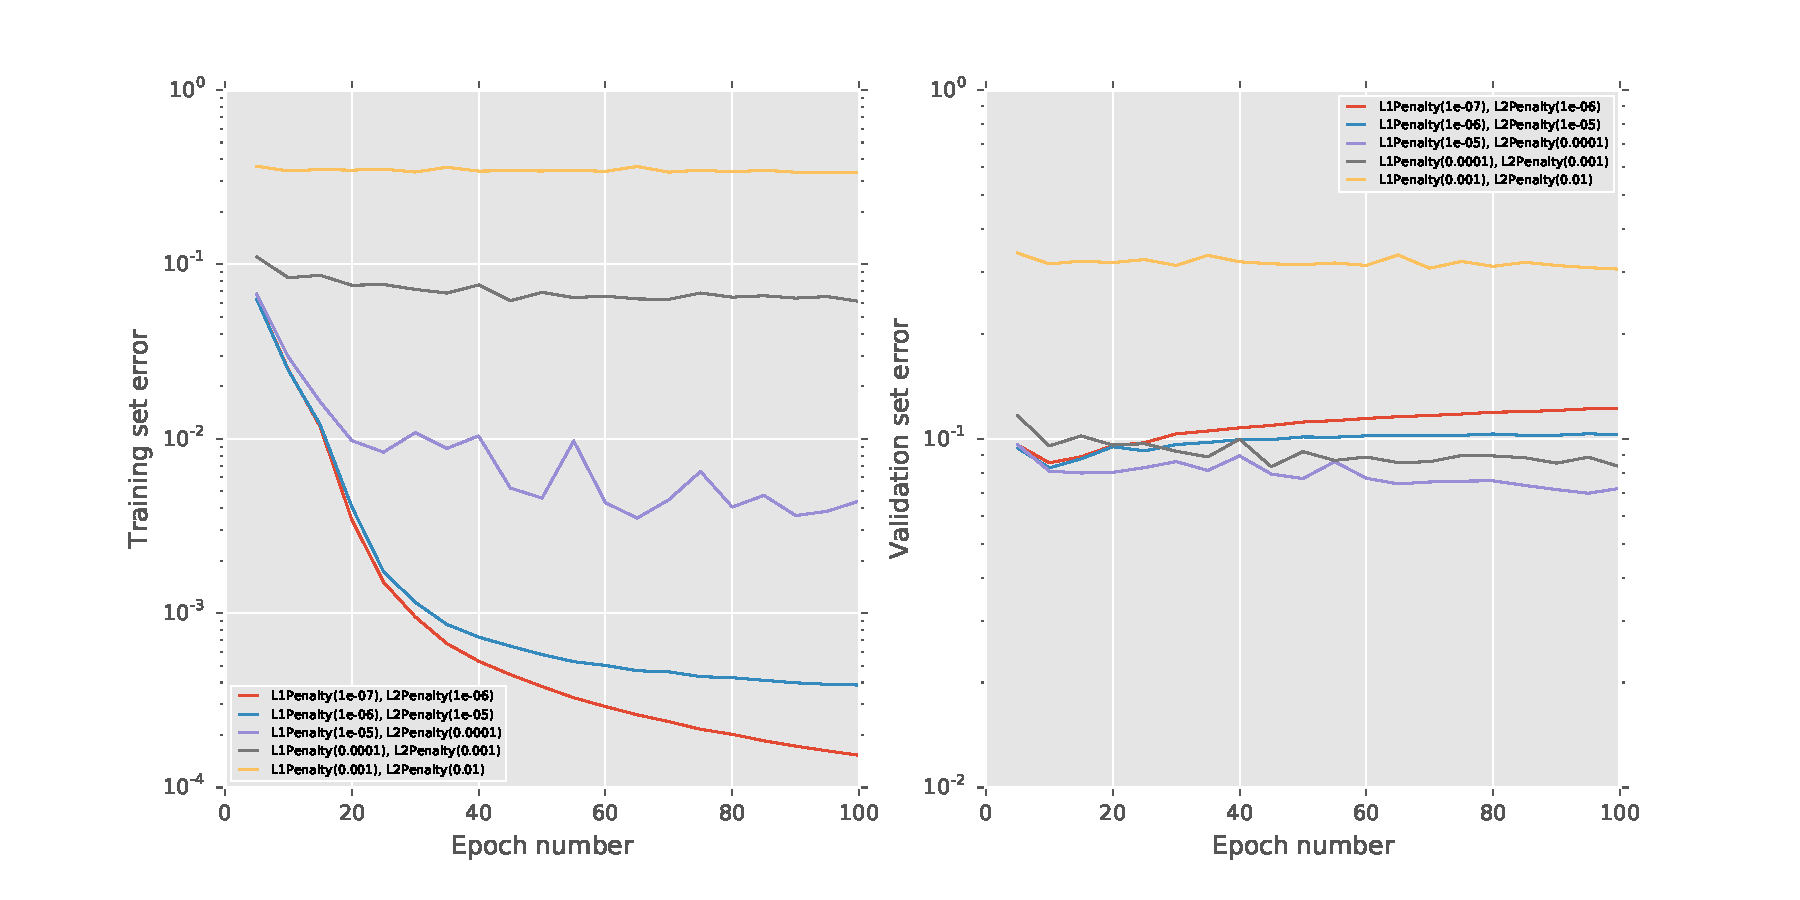
\includegraphics[width=1\textwidth]{L1_L2.pdf}
  \caption{training error and validation error for L1 and L2 combination method}
  \label{fg:L1_L2_combine}
\end{figure}

\begin{table}
\begin{center}
\begin{tabular}{ c  c c c c  c c} 
\hline
coeff\_L1 & coeff\_L2 &error(train) & error(valid) & acc(train) & acc(valid) & params\_penalty\\
\hline
\hline
None & None	&1.53e-04 & 1.22e-01 & 1.00e+00 & 9.79e-01 &7.05e-04\\ 
1e-06 & 1e-05  	&3.87e-04 & 1.03e-01 & 1.00e+00 & 9.80e-01 &5.81e-03\\ 
1e-05 &1e-04	 &4.39e-03 & 7.21e-02 & 1.00e+00 & 9.80e-01 &3.38e-02\\ 
1e-04 & 1e-03 & 6.13e-02  &  8.31e-02  &  9.83e-01 & 9.76e-01  &  1.39e-01\\
1e-03 & 1e-02 &3.37e-01&  3.06e-01   & 9.09e-01 & 9.21e-01 &4.13e-01\\
\end{tabular}
\caption{Performance of different coefficients for combining method for L1 and L2}
\label{tb:L1_L2_combine}
\end{center}	
\end{table}

\begin{figure}[h]
\centering 
  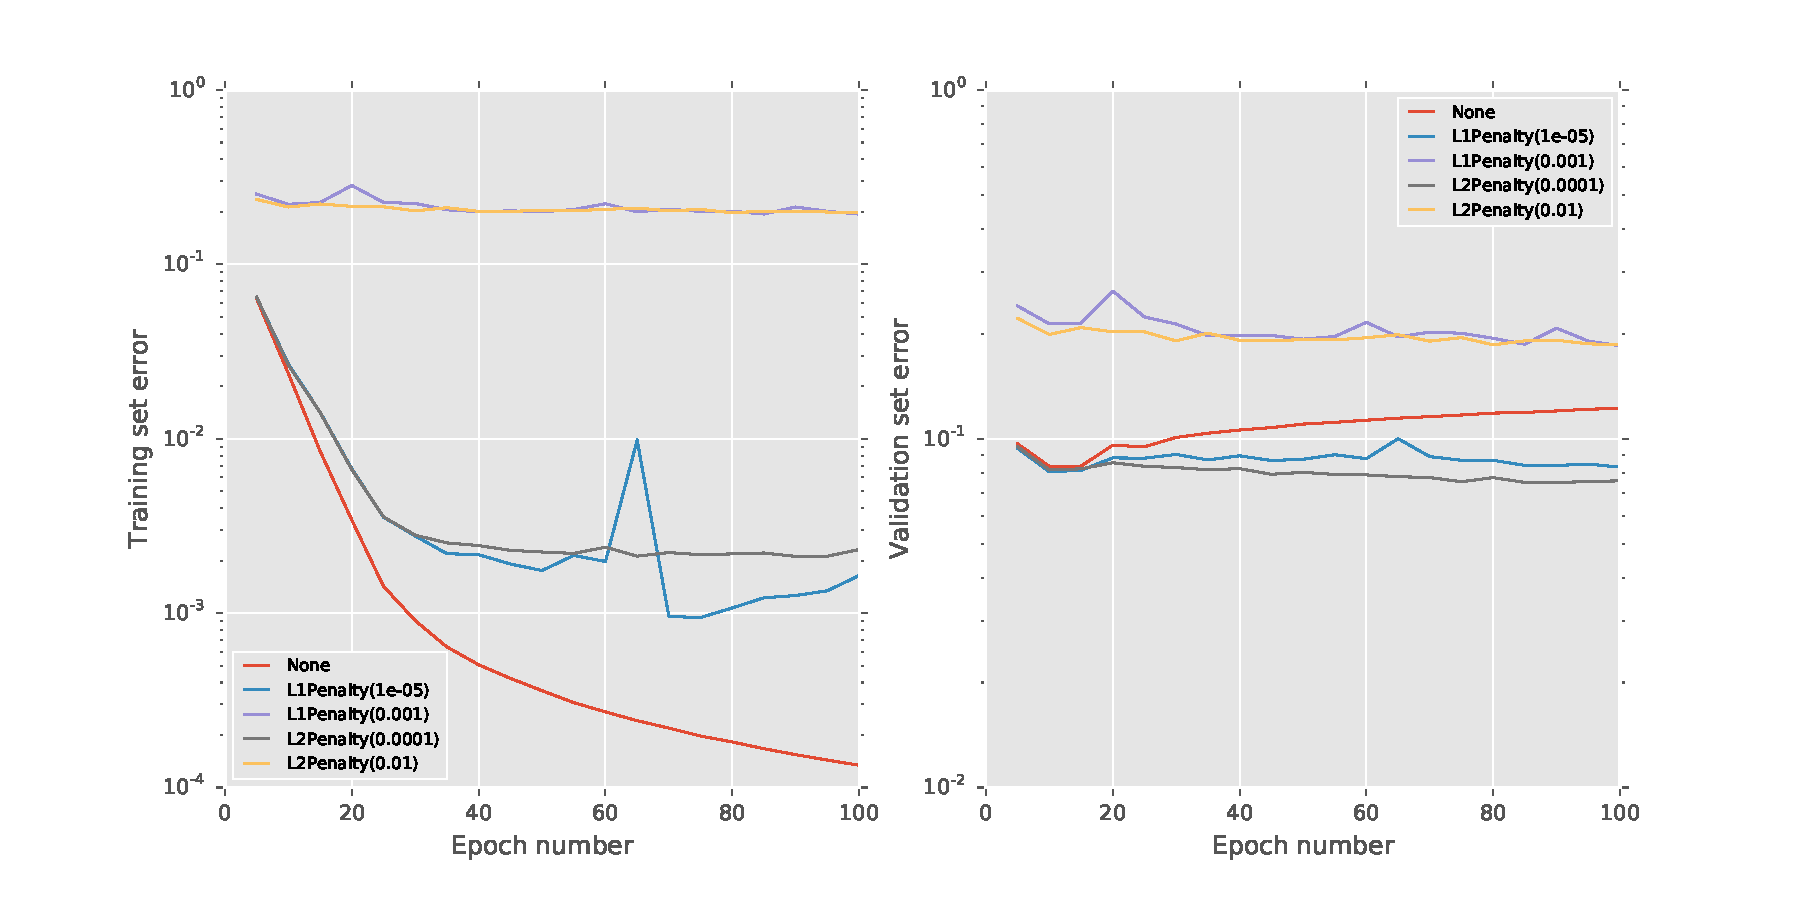
\includegraphics[width=1\textwidth]{baseline_L1_L2.pdf}
  \caption{training error and validation error for L1 and L2 combination method}
  \label{fg:L1_L2_combine}
\end{figure}

\subsection{Discussion and Conclusion}
From the Table \ref{tb:L1_L2_combine}, it can be shown that the smallest validation error is achieved when coefficient for L1 is $1e-05$ and coefficient for L2 is $1e-04$. The parameters penalty is neither too high nor too lower so that the model will not overfitting nor underfitting. For larger coefficients the parameters penalty is too large so that the speed of learning is very slow. However, For smaller coefficients, the validation error starts to increase with the decreasing of training error, which indicates a overfitting problem. On reason for that could be the relatively small value of coefficients on L1 and L2 term so that the effects of penalty is minor.


\newpage
\section{Data Augmentation}
\subsection{Experimental hypothesis}
Several ways was investigated to expand the training data such as rotating, zooming of existing data and elastic deformation \cite{Elastic}. In this experiment, we are going to find wether adding distorted inputs to training data could produce better performance on testing and how well does these ways behaves on testing sets.
\printbibliography
\end{document}